\documentclass{seminar}
%\documentclass[german]{seminar}

\usepackage{tikz}
\usepackage{booktabs}
\usepackage{multirow}
\usepackage{url}
\usepackage{enumitem}
\usepackage{wrapfig}
\usepackage{lipsum}
\usepackage{colortbl}
\usetikzlibrary{shapes,arrows}

\newcommand{\q}[1]{``#1''}
\newcommand{\tabitem}{~~\llap{\textbullet}~~}
\newcommand{\exampleQuote}[1]{\small{\textit{``#1''}}}
\newcommand{\obsrvQuote}[1]{\textit{``#1''} }
\newcommand{\red}[1]{{\color{red}#1}}
\hyphenation{PICOT}
\hyphenation{FINER}
\hyphenation{EBSE}


\begin{document}

%\semcover{Make studies great again!}
\semcover{A structured approach to evidence-based software engineering in empirical software engineering research for students}
	{M. Danz, T. Gr\"af, C. Michel}
	{danz@teco.edu, tobias.graef@student.kit.edu, michel@teco.edu}
	{Andrei Miclaus}
	{miclaus@teco.edu}


\newpage
% !TEX root = ../../seminar.tex

\begin{abstract}
~\\\\\textbf{Background}: It was found, that some students struggle with scientific working.\\
\textbf{Objective}: Create a supporting document tailored for students. With a main focus on ease of use and with EBSE in mind to establish it further.\\
\textbf{Results}: Based on literature and experience, a process and supporting documents are created. The process is based on EBSE. To make the document easy to use, it incorporates simple and clear design as well as concise instructions.\\
\textbf{Limitations}: This work is mainly aimed at computer science students and needs to be evaluated in future work.

\semkeywords{
software engineering, 
evidence-based software engineering,
EBSE,
scientific working,
flowchart,
checklist,
student workflow}

\end{abstract}

\newpage
\setcounter{tocdepth}{3}
\tableofcontents

\newpage
Final TODOs:\\
\todo{check for broken quotes}\\
\todo{check figure references}\\
\todo{check section references}\\
\todo{fix ToC chapter }\\
\todo{add appendix and reference to it}\\
\todo{check for first term occurence with using italic text}

\newpage
% !TEX root = ../../seminar.tex


\section{Introduction}
\label{sec:introduction}

It was observed\todosoft{rephrase} that most software build in a bachelor's or master's thesis is poorly evaluated or not evaluated at all. Therefore our initial aim was finding or creating a method to evaluate and compare software suited for students.

But we soon discovered a major problem: Large pieces of software are hard to evaluate because effects can be hard to isolate.
To find out which software \todosoft{SW architecture, devel method..} is more suitable for a given problem, measurements are needed for a quantitative comparison. Moreover, a controlled study is needed to attain valid measurements that allow comparison. Students often struggle with obtaining this \emph{empirical evidence} (see table \ref{table:issuesEBSE}) leading to unusable results making a proper comparison difficult or not possible at all. 

So we revised the question to: How to create a supporting system for students helping to improve the quality (in particular the substantiality) of their studies in the domain of software engineering.

The final system we intend is an electronical\todosoft{digital? should this be here or just in dicussion because it is not actually part of this paper.} database containing a collection of experiments. The system is meant to simplify searching, scanning and comparison of experiments. Allowing to quickly find existing evidence that can be used for software design decisions. To populate that collection, a process to create evidence correctly and a compact representation of the results are needed. We propose two documents: \emph{\checklist} to guide students through the scientific process and \emph{\briefingform} for a compact, structured and complete resume of the conducted experiment. 


\todo{rest of chapter are notes:}
\begin{itemize}
\item experimentation/empiricism in CS?
\item \q{should computer scientists experiment more?, Tichy 1997}
\item Experimental evaluation in CS: A quantitative study, 1994: 40\% of papers requiring quant evaluation have none (other disciplins: 15\%)
\item \q{A survey of Controlled Experiments in SE, 2005} from 1993 to 2002: 1,9\% of software engineering paper report controlled experiments
\item \q{Belief \& Evidence in Empirical Software Engineering}, 2016: programmers have strong beliefs, primarily formed by personal opinion (research papers just above "other", below peer opinion, mentor opinion and trade journals); beliefs vary between projects, but do not necessarily correspond with evidence in that project
\item \q{Incorrect results in software engineering experiments: How to improve research practices}, 2016: research and publication bias quite common, need to improve research practices (a key: avoid experiments with low statistical power)
\end{itemize}


In section \ref{sec:related work} \emph{evidence-based software engineering} (EBSE) and structured abstracts are introduced. EBSE is the foundation of the process introduced later in section \ref{sec:research process}. Therefore, the idea behind EBSE is very fundamental  for this paper.\\
Structured abstracts are used as a base for the form introduced in section \ref{sec:briefing form}.\\

















\newpage
% !TEX root = ../../seminar.tex

\section {Fundamental Principles}
\label{sec:fundamental principles}
In this section, \emph{evidence-based software engineering} (EBSE) and structured abstracts are introduced. EBSE is the foundation of the process introduced later in section \ref{sec:research process}. Therefore, the idea behind EBSE is very fundamental  for this paper.\\
Structured abstracts are used as a base for the form introduced in section \ref{sec:briefing form}.\\
\todo{more text?}
	% !TEX root = ../../seminar.tex

\subsection{EBSE}
\label{subsec:EBSE}

\todosoft{short introduction to EBSE,...}
\newline
In 2004 evidence-based software engineering (EBSE) was proposed as an adoption of the evidence-based approach in medicine \cite{EBSE}. The aim of EBSE is \q{to improve decision making related to software development and maintenance by integrating current best evidence from research with practical experience and human values} \cite{Dyba2005}. Practising EBSE includes five steps:
\begin{enumerate}
	\item Ask an answerable question.
	\item Find the best evidence that answers that question.
	\item Critically appraise this evidence.
	\item Apply the evidence (and critical appraisal).
	\item Evaluate the performance in previous steps.
\end{enumerate}
Formulating the question precisely is important for the success of the process. The question should be formulated broad enough, so important studies are not missed, but must be precise enough to cope with the amount of studies (see section \ref{subsec:formulating research question and hypothesis}).

In medicine researcher heavily rely on already published \emph{systematic literature reviews} (SLR) to find relevant studies. SLRs try to identify and interpret all available literature regarding a specific research question \cite{keele2007}. There are several organisation dedicated to conduct such reviews in medicine. The lack of this infrastructure makes applying the evidence-based approach in software engineering more difficult, but the number of existing SLRs increases steadily.

It is important to check the quality of the identified studies, because being published is not a guarantee for good research. Sometimes one cannot trust the results, because the research method has weaknesses or the researcher has vested interest connected to the outcome of the study.

Applying the evaluated evidence means integrating it with personal experience and other requirements. This step highly depends on the context and type of technology under evaluation.

At last the performance in previous steps is evaluated to improve applications  of the EBSE process in the future.

Kitchenham \etal \cite{EBSE} also identify two major problems inherent to software engineering:
\begin{enumerate}
\item The skill factor: Performing software engineering methods and techniques often require skilled practitioners. This prevents blinding and can therefore cause problems related to subect and experimenter bias.
\item The lifecycle issue: Prediction of behaviour \todosoft{long time?} of deployed technology is difficult and it is hard to isolate efffects because of interaction with other methods and technologies.
\end{enumerate}

They also state two approaches to reduce each of these effects we do not want to discuss here.
\todosoft{do not mention these approaches?}	 



	% !TEX root = ../../seminar.tex

\subsection{Structured Abstract}
\label{subsec:structured abstract}

In their guidelines for reporting experiments in software engineering Jedlitschka \etal \cite{Jedlitschka2008} propose the use of \emph{structured abstracts}. They adopted the idea from medicine and psychology, where structured abstracts were introduced to increase the quality of abstracts. Structured abstracts guide the writer as well as the reader by using headings. Although a variety of different elements is used (see for example \todo{} \q{Adoption of structured abstracts by general medical journals and format for a structured abstract
}), the most common elements of structured abstracts are \emph{Background/Context}, \emph{Objective/Aim}, \emph{Methods}, \emph{Results} and \emph{Conclusion/Discussion}. Jedlitschka \etal \cite{Jedlitschka2008} suggest the use of a sixth heading called \emph{limitations}. This information is necessary to decide whether a result can be transfered to another context. Kitchenham \etal \cite{KBO2008} include this information in the \emph{conclusion} section.

The list and description of elements below closely follows the suggestion of Jedlitschka \etal \cite{Jedlitschka2008}:
\begin{enumerate}
	\item \emph{Background/Context}: Briefly explains the motivation for conducting the study and refers to previous research.
	\item \emph{Objective/Aim}: Describes the purpose of the study, including the object that is studied as well as focus and perspective. This part should cover the research question.
	\item \emph{Methods}: Sums up used research methods. For example experimental design, setting, participants and selection criteria, intervention and measurement and analyzing technique.
	\item \emph{Results}: The key findings are described here in form of numerical values. Do not include interpretations here. See section \ref{statisticalresults} (Statistical Results) for further details.
	\item \emph{Limitations}: Describes the scope  of the study to point out the limits of generalization. This element might be incorporated in the \emph{conclusion}-element.
	\item \emph{Conclusion}:  Contains the interpretation of results and puts them into larger context.
\end{enumerate}

%Additionally, keywords can be used for a quick overview. They can also help to find work easier using search engines.

There are several studies comparing structured and unstructured abstracts in the domain of software engineering with regard to completeness and clarity:
\begin{itemize}
\item Structured abstracts include more relevant information and are easier to read than conventional abstracts \cite{Budgen2007,Budgen2008}.
\item Inexperienced authors are likely to produce clearer and more complete abstracts when using a structured form \cite{Budgen2011} .
\item On average structured abstracts are longer (limitations in conclusion is a good idea to prevent lengthy abstracts) and have better readability than unstructured abstracts \cite{KBO2008}.
\end{itemize}
	
These findings are consistent with the ones in other disciplines. It is important to mention that there are critics of structured abstracts that are supported by studies, but in general structured abstracts are considered advantageous \cite{hartley2004,hartley2014}.	

A downside to structured abstracts is their length compared to unstructured ones. If the size of abstracts is limited, the abstract should still be in a structured form traditional elements should be prioritized: background (one sentence), objective, methods, result and conclusion \cite{Jedlitschka2008}.

If it is not possible to structure an abstract (e.g. due to standard of journal or supervisor, length limitations) the elements of a structured abstracts should be contained in the unstructured abstract to make sure no important information is missing. See the common structure of the clearest abstracts as found by Shaw \cite{shaw2003}. Moreover the reader should be able to quickly identify each element by reading through the abstract.

For further information  and examples of structured abstracts see the guide of C. Andrade \cite{Andrade2011} and Kitchenham \etal \cite{EBSE}.


\newpage
% !TEX root = ../../seminar.tex

\section{Related Work}
\label{sec:related work}
\todosoft{einleitung}

Rainer \etal \cite{Rainer2006} released a paper about the reported use of EBSE by 15 under-graduate students. 
We have used observations listed in the paper to create design guidelines for the documents introduced in section \ref{sec:research process} and \ref{sec:briefing form} . There are seven main issues we tried to address:
% !TEX root = ../../seminar.tex
\begin{table}
	\begin{enumerate}
		\item \label{itm:issue1} \q{Students had problems constructing well-formulated EBSE questions.}
		\item \label{itm:issue2} \q{Students used limited criteria for identifying the best or better evidence [\ldots]}
		\item \label{itm:issue3} \q{Students used a very limited number of search terms.}
		\item \label{itm:issue4} \q{Students provided poor explanation in their reports of how their searches were conducted.}
		\item \label{itm:issue5} \q{Students varied in their use of the EBSE checklist.}
		\item \label{itm:issue6} \q{Some students critically appraised the technologies rather than the publications (evidence) on the technologies.}
		\item \label{itm:issue7} \q{But we also think that the kinds of problems students were tackling [\ldots] are not the kinds of problems researchers commonly investigate.}
	\end{enumerate}
	\caption{Issues with EBSE found by Rainer \etal\cite{Rainer2006}}
	\label{table:issuesEBSE}
\end{table}

\todo{mention? some of these issues addressed in \q{Using systematic reviews and evidence-based software engineering with masters students}}\\

SEED\todo{ref paper} and the \emph{Evidence Map}\footnote{\url{http://community.dur.ac.uk/ebse/}} \todo{paper exists?, ref} are databases that are meant to ease the access to studies.\\ 
SEED is a community-driven online database that has been created during graduate courses. It lists summaries of studies in a common format and grouped by topics. The studies are added by researchers, whereas users create summaries, ratings and comparison grids. There only exists a prototype\footnote{\url{http://evidencebasedse.com}} that has not been updated since 2009.\todo{criticise format of study representation?}\\
The Evidence Map is primarily concerned with  classifying systematic literature reviews (secondary studies, see sections \ref{subsec:EBSE} and \ref{subsec:search for existing evidence}), but also provides lists of primary and tertiary studies as well as information and guidelines about EBSE. A major disadvantage is the lack of study summaries. It has not been updated since 2012.

\todo{Large graph} \cite{Rainer2008}


\newpage
% !TEX root = ../../seminar.tex

\section{Student Process Improvement Document - \checklist}
\label{sec:research process}

\begin{minipage}{\linewidth}
\begin{wrapfigure}{R}{0.3\textwidth}
	\centering
	\vspace{-1.0cm}
	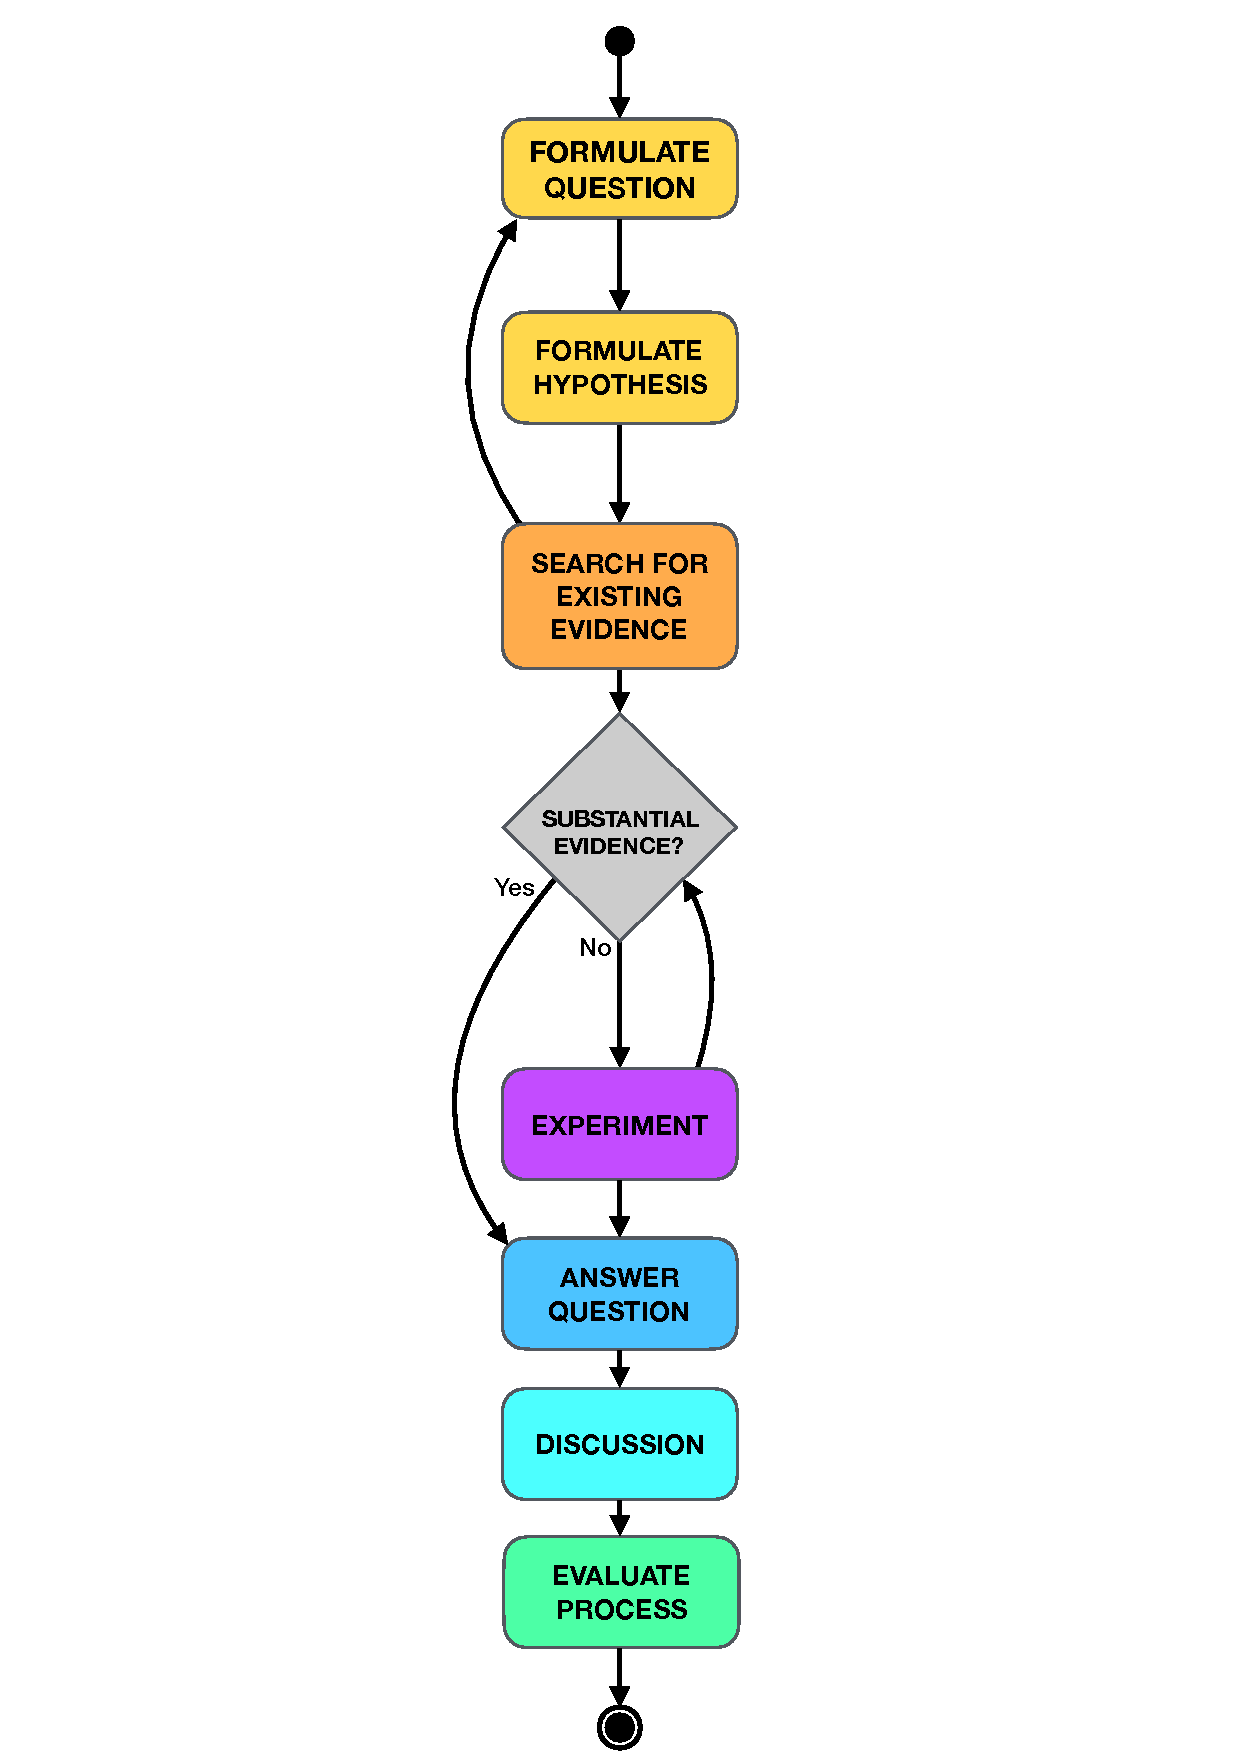
\includegraphics[trim={3cm 0 3cm 0}, height=14.55cm]{figures/workflow_graph.pdf}
	\caption{Workflow Graph}
	\label{fig:workflow_graph}
\end{wrapfigure}


In this section, a document called \emph{Student Process Improvement Document (\checklist{})} is introduced. It is supposed to guide students through scientific working with EBSE in mind.

Rainer \etal found, that \q{[s]tudents varied in their use of the EBSE checklist} \cite{Rainer2006} (see issue \ref{itm:issue5} in table \ref{table:issuesEBSE}). Therefore, an important design criteria for \checklist{} is ease of use through clear and simple instructions. Especially tailored for students with little knowledge about scientific working in general.

The process of \checklist{} contains eight steps:
\begin{enumerate}
\item Formulate question
\item Formulate hypothesis
\item Search for existing evidence
\item Substantial evidence
\item Experiment
\item Answer question
\item Discussion
\item Evaluate process
\end{enumerate}


The whole graph can be seen in figure \ref{fig:workflow_graph}. The actual document can be found in appendix \ref{appendix:checklist}.\\
On the left of the document, a flow chart of the proposed process is depicted. For computer science students this should be a fast way to navigate through and orient themselves in the process. To further assist navigation visually, each process step has been assigned a unique color. This color schemes reoccurs in the tools section of the document as well as in \briefingform.

On the right additional information is given. Each process step in \checklist{} contains a short description, some guidelines, and acceptance criteria. The guidelines contain methods and tools on how to process the current step. The acceptance criteria give students orientation on when a step is completed.
\end{minipage}










	% !TEX root = ../../seminar.tex

\subsection {Scientific Method}
\label{subsec:scientific method}

The scientific method is a model which describes the working process of scientific working in general. In figure \ref{fig:SCIENTIFIC_METHOD}, the \checklist{} process is mapped on the scientific method. The colors indicate which steps of \checklist{} correspond to which steps of the scientific process. \\
A large part of the scientific method is focused on finding research topics (white) and formulating research questions (yellow). In contrast \checklist{} focuses on answering the research question. This is represented by multiple colors being mapped onto only two steps and two transitions in figure  \ref{fig:SCIENTIFIC_METHOD}. The steps marked white are not contained in \checklist{}.
The different focuses are caused by advisors usually assigning students a narrow research topic or a specific research question.

\begin{figure}
	\centering
	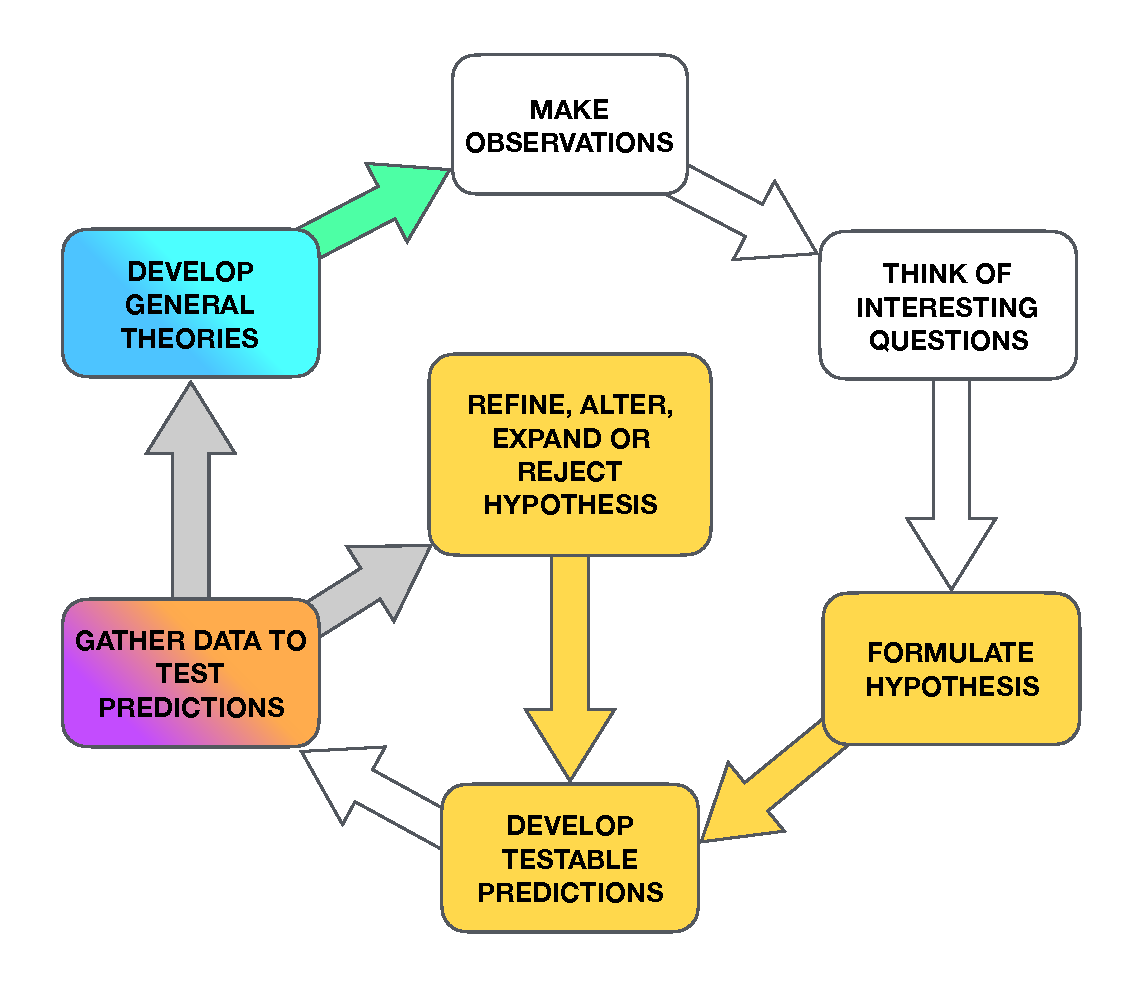
\includegraphics[width=12cm]{figures/scientific_method_mapping.pdf}
	\caption{Mapping of our process to the scientific method \cite{ScienceMethod}.}
	\label{fig:SCIENTIFIC_METHOD}
\end{figure}



	\subsection{Formulating Research Question and Hypothesis}
\label{subsec:formulating research question and hypothesis}

For researchers to produce relevant results and understand their research domain fully, the step of developing a good research question, with a supporting hypothesis and sometimes objectives is integral \cite{Farrugia2009}. These components should be carefully designed \emph{before} conducting the study that tries to answer the question. Otherwise it is more likely to produce questions that are already answered, or \q{could potentially lead to spuriously positive findings of association through chance alone.} \cite[p. 280]{Farrugia2009} 

		\subsubsection{Research Question}

The question the later study is designed to answer is called research question \cite{Vickers}. It should be an answerable question and address a relevant issue in the research area \cite{Dyba2005}. Preceding a research question is the need for a deep understanding of the topics that have already been studied, in order to produce questions which drive knowledge further. The questions that arise during the acquisition of knowledge, and cannot be answered by means of EBSE, are likely appropriate questions for further research \cite{Farrugia2009}. \newline
There are two general classes of research questions: qualitative and quantitative questions. Qualitative research states questions which report, describe, or explore a subject \cite[p. 139-141]{Creswell2014}. In computer science as the research field matures these questions become more and more rare {\color{red} (find source)}. Therefore focus is on quantitative research questions in this paper. \obsrvQuote{Quantitative research questions inquire about the relationships among variables} \cite[p. 143]{Creswell2014}, and from them emerge quantitative hypotheses. \newline
To understand the structure of research questions Shaw provides a model where she categorizes research questions from software engineering papers in five types \cite{Shaw2002} {\color{red} (maybe cut out)}. \newline
To design a good research question Haynes coined the acronym PICO: Population, Intervention, Comparison group, and Outcome \cite{BrianHaynes2006}. Sometimes Time is added as fifth component, when it is important over what time frame the study is conducted, see Table \ref{table:PICOT}. A research question structured with the PICOT approach supports in restricting the research question and steers thereby hypotheses and study. By restricting the research question researchers can limit bias and increase the internal validity of the study, but a too narrow question may also lead to decreased external validity \cite{Farrugia2009}. \\
Before PICOT Sackett and colleagues suggested that good research questions consist out of three components: Intervention, Context and Outcome \cite{Sackett2000}, which is a more coarse grained decomposition than PICOT. Dyb{\aa} \emph{et al.} displayed a fitting example for this template in software engineering: \obsrvQuote{Does pair programming lead to improved code quality when practiced by professional software developers?} \cite[p. 60]{Dyba2005} Here the intervention is pair programming, the context of interest are professional software developers, and the outcome is improved code quality \cite{Dyba2005}. To verify the quality of a freshly designed research question Hulley \emph{et al.} suggest the use of the FINER criteria. It highlights key aspects of the question and provides thereby new angles to view the proposed study from. The FINER criteria consists of: Feasible, Interesting, Novel, Ethical, and Relevant \cite{Farrugia2009}. A more detailed view of the FINER criteria can be seen in Table \ref{table:FINER}. {\color{red}(TODO specify more tips for writing a good question. Creswell2014)}  


\begin{table}[]
	\centering
	\fbox{
		\begin{tabular}{ p{3em} p{6.5em} p{22em} }
			\textbf{P}	& Population & What specific population are you interested in? \vspace{1em}\\
			
			\textbf{I}	& Intervention (technology) & What is the investigational technology/ intervention? \vspace{1em}\\
			
			\textbf{C}	& Comparison group & What is the main alternative/baseline to compare with the intervention \vspace{1em}\\ 
			
			\textbf{O}	& Outcome & What do you intend to accomplish, measure, improve or affect? \vspace{1em}\\ 
			
			\textbf{T}	& Time & What is the appropriate follow-up time to assess outcome? 
		\end{tabular}	
	}
	\vspace{1em}
	\caption{PICOT criteria adjusted to fit better in computer science research.}
	\label{table:PICOT}
\end{table}

\begin{table}[]
	\centering
	\fbox{
		\begin{tabular}{ p{3em} p{6em} p{22em} }
				\textbf{F}	& Feasible & \tabitem Adequate number of subjects \\
				\multicolumn{2}{l}{} & \tabitem Adequate technical expertise \\
				\multicolumn{2}{l}{} & \tabitem Affordable in time and money \\
				\multicolumn{2}{l}{} & \tabitem Manageable in scope \vspace{1em}\\
				\textbf{I}	& Interesting & \tabitem Getting the answer intrigues investigator, peers and community \vspace{1em}\\
	
				\textbf{N}	& Novel & \tabitem Confirms, refutes or extends previous findings \vspace{1em}\\
	
				\textbf{E}	& Ethical & \tabitem Amendable to a study that institutional review board will approve \vspace{1em}\\ 
				\textbf{R}	& Relevant & \tabitem To scientific knowledge \\
				\multicolumn{2}{l}{} & \tabitem To clinical and health policy \\
				\multicolumn{2}{l}{} & \tabitem To future research
		\end{tabular}	
	}
	\vspace{1em}
	\caption{FINER criteria for a good research question \cite{Farrugia2009}}
	\label{table:FINER}
\end{table}




		\subsubsection{Hypothesis}

\begin{itemize}
	\item What is it?
	\item For what is it?
	\item is testable statement  {\color{red} (find source)}
	\item Only in Quantitative research  {\color{red} (Creswell)}
	\item two-sided/one-sided hypothesis -> use only two-sided  {\color{red} (Farrugia et al.)}
	\item Null hypothesis in empirical work  {\color{red} (Farrugia et al.)}
	\item contains varaibales/population/relationship  {\color{red} (health website)}
	\item How to hypothesis:
	\begin{itemize}
		\item  {\color{red} (Prasad)}
		\item from websites  {\color{red} (find sources)}
		\item  {\color{red} (Creswell)}
	\end{itemize}
\end{itemize}
		\subsubsection{Objectives}

 Sometimes researchers define objectives to their hypotheses. They are active statements that \obsrvQuote{define specific aims of the study and should be clearly stated} \cite[p. 280]{Farrugia2009} at the beginning of research. Objectives help to define the study (e.g. helping to calculate sample size). \cite{Farrugia2009,Vickers} Although we do not include objectives in our \briefingform we would like to mention them for reasons of completeness.
	% !TEX root = ../../seminar.tex

\subsection{Search for Existing Evidence}
\label{subsec:search for existing evidence} 

After formulating a research question it is important to know which scientific results exist that help answer this question. Students normally perform an \q{ad-hoc} literature review that is prone to missing evidence and getting biased results (experimenter bias).

For that reason EBSE proposes the use of \emph{systematic literature reviews} (SLR), a type of secondary study, to search for studies related to the research question. The aim of SLRs is to \q{identify, assess and combine the evidence from primary research studies using an explicit and rigorous method} \cite{Zhang2011}. Using this well-defined method might prevent biased results of the literature review, but requires more effort (both in time and skill) than traditional literature reviews. There exist guidelines \cite{keele2007,Wohlin2014,Zhang2011} and reports of experiences with conducting SLRs \cite{Brereton2007} that provide the means necessary to conduct a SLR.

In any case published SLRs are very useful, even if conducting one is not feasible, as they provide a summary of multiple studies concerning one research question. Currently there are at least two projects concerned with making SLRs and finding relevant studies easier by collecting and indexing them \todo{ref SEED and Software Engineering Evidence Map}, but both have not been updated recently \todo{(SEED: prototype, 2009; Ev Map 2012)}. \todosoft{more disadv?}

Students voted for the SLR conducted during the EBSE process as one of the hardest steps \cite{keele2007}. Therefore we suggest a less formal search process to save time and effort. But it should be noted, that the search should still be planned and structured to get the desired result\todosoft{state it?}. If it is possible conducting a SLR is always preferable.
\newline
\newline
Several guidelines from SLRs are still useful \todosoft{rephrase}:
\begin{itemize}
\item Think about your search strings and engines beforehand and write them down. This also addresses issue \ref{itm:issue4} (see section \ref{sec:related work}).
\item It is unlikely to find all relevant literature using only a single search engine \cite{Brereton2007}. \todosoft{GS as good starting point (publisher bias)?}
\item \emph{Snowballing} is useful, both in a forward and backward manner \cite{Wohlin2014}.

\emph{Backward}-snowballing refers to looking at the references of a publication an therefore going back in time. This can be done by using the \q{cited by} functionality of Google Scholar.

\emph{Forward}-snowballing means going forward in time by looking at the papers citing the current paper.
\item The search strategy depends on the research question. If the research domain provides a vast amount of studies the search can \todosoft{should, must?} be restricted, for example the exclusion of older studies \cite{Brereton2007}.
\item Even for more experienced students it might be necessary to refine the research question based on the search result, because their understanding of the research domain increases \cite{Brereton2007}. For example having only a few search result can be caused by research questions that are too narrow. Research Questions that are too general can lead to an abundance of search result that would take too long to examine \todosoft{or can't be handled?}. 
\item Categorize your research question using classification systems like the ACM Computing Classification System and search within these categories. This is especially helpful if it is problematic to limit the scope with in the research area or there are uncertainties about wording and naming\todosoft{rephrase}
\end{itemize} 

\todo{issue \ref{itm:issue3}?}

\todosoft{
mention? systematic mapping studies (broader, but not as deep as SLRs (deep: quantitative analysis and quality assessment))
\q{Systematic Mapping Studies in
Software Engineering}, Petersen \etal 2008
}
	% !TEX root = ../../seminar.tex

\subsection{Designing, Conducting And Interpreting Experiment}
\label{subsec:designing conducting and interpreting experiment}
To generate evidence, experiments are conducted. To keep the complexity of the study manageable and prevent side effects, it is recommended to answer only one question per experiment. If the question is too extensive for a single experiment, split up the question in sub-questions and recursively start this process with each sub-question.\\
For guidance and documentation through the experiment use \briefingform introduced in section \ref{sec:briefing form}. Since experimenting is a very complex topic and can not be fully covered in this paper, see \cite{Wohlin2012,Tullis2013} for further reading.
	% !TEX root = ../../seminar.tex

\subsection{Answer Question}
\label{subsec:answer question}

Before you can answer a question the existing studies must be critically appraised. This means checking the study design, study quality, relevance for the research question, as well as consistency between different studies. 

The \emph{GRADE approach} \cite{Atkins2004} is a grading system for studies that goes beyond simple hierarchies of study types. It was introduced for medicine and has been used in the software engineering domain \cite{Wohlin2013EvidenceProfile,Dyba2008}. It is a well-defined method and differentiates between the quality of evidence and the strength of recommendation. Figure \ref{fig:critical appraisal} shows a checklist containing the important factors to consider when appraising a study and we suggest following it when appraising studies.

\begin{figure}[h]
\fbox{\parbox{\textwidth}{
\large
\textbf{Study Appraisal Checklist}
\normalsize
\begin{enumerate}
\item \textbf{Is there any vested interest?}
	\begin{itemize}
	\item Who sponsored the study?
	\item Do the researchers have any vested interest in the results?
	\end{itemize}
\item \textbf{Is the evidence valid?}
	\begin{itemize}
	\item Was the study’s design appropriate to answer the question?
	\item How were the tasks, subjects, and setting selected?
	\item What data was collected, and what were the methods for collecting the data?
	\item Which methods of data analysis were used, and were they appropriate?
	\end{itemize}
\item \textbf{Is the evidence important?}
	\begin{itemize}
	\item What were the study’s results?
	\item Are the results credible, and, if so, how accurate are they?
	\item What conclusions were drawn, and are they justified by the results?
	\item Are the results of practical and statistical significance?
	\end{itemize}
\item \textbf{Can the evidence be used in practice?}
	\begin{itemize}
	\item Are the study’s findings transferable to other industrial settings?
	\item Did the study evaluate all the important outcome measures?
	\item Does the study provide guidelines for practice based on the results?
	\item Are the guidelines well described and easy to use?
	\item Will the benefits of using the guidelines outweigh the costs?
	\end{itemize}
\item \textbf{Is the evidence in this study consistent with the evidence in other available studies?}
	\begin{itemize}
	\item Are there good reasons for any apparent inconsistencies?
	\item Have the reasons for any disagreements been investigated?
	\end{itemize}
\end{enumerate}
}}
\caption{Checklist for critical appraisal of studies compiled by Dyb{\aa} \etal \cite{Dyba2005}}
\label{fig:critical appraisal}
\end{figure}

One important aspect of appraising studies is checking whether they might be biased. J{\o}rgensen \etal \cite{Jorgensen2016} reported indications of research and publication bias being quite common in the domain of software engineering. Shepperd makes similar findings and gives a good and short overview of the problem \cite{Shepperd2015}.

The hypothesis is accepted or rejected on the basis of the critical appraisal and the research question is answered accordingly.

\todo{text}\\
- Evidence Substantial? For Evidence classification maybe quote:\\
\cite{Wohlin2013EvidenceProfile} or \\
\url{https://www.researchgate.net/publication/305632179_Evidence-based_software_engineering} (\q{Strength of Evidence}) \textit{(mendeley import adds wrong meta-data, therefor just an url and not an actual reference yet)}\\
- maybe reference to different types of bias\\
- make sure evidence fits to the question\\
- accept or reject hypothesis\\
- answer research question accordingly\\

	% !TEX root = ../../seminar.tex

\subsection{Discussion}
\label{subsec:discussion}
\todosoft{Text}
Discuss the whole study, suggest future approaches and limits. Put study in larger context and explicitly  scope of generalization.
Analyze your study using the checklist in figure \ref{fig:critical appraisal}.
Make sure, to only discuss the content of the study. To reflect the process, see section \ref{subsec:evaluate process}.
	% !TEX root = ../../seminar.tex

\subsection{Evaluate Process}
\label{subsec:evaluate process}

The last step of the process proposed here is to reflect on the process itself. After discussing the study and finishing it in the step before (see section \ref{subsec:discussion}), Dyb{\aa} \etal recommend to reflect on how well each step was performed and what could be improved in the next iteration. To support this they recommend using \emph{after-action reviews} (AAR) and \emph{postmortem analysis} (PMA) \cite{Dyba2005}.

AAR is a short meeting of 10 to 20 minutes answering the four questions in figure \ref{fig:aar_pma}, left box. This method can also be used at any other point the process when need is to reflect on or rethink the current situation\cite{Dyba2005}.

PMA is similar to AAR but with a deeper insight. Therefore it lasts for several hours up to a full day. It answers the questions in figure \ref{fig:aar_pma}, right box \cite{Dyba2005}. Here conclusions can be drawn to improve upcoming EBSE cycles and further research in general. This method can give insight issues like: which methods worked out as planned and which did not. Where was time lost and deadlines missed. Which technique proves to be used in upcoming studies. 

After this step the whole process starts over again with the next research question.

\begin{figure}
	\centering
	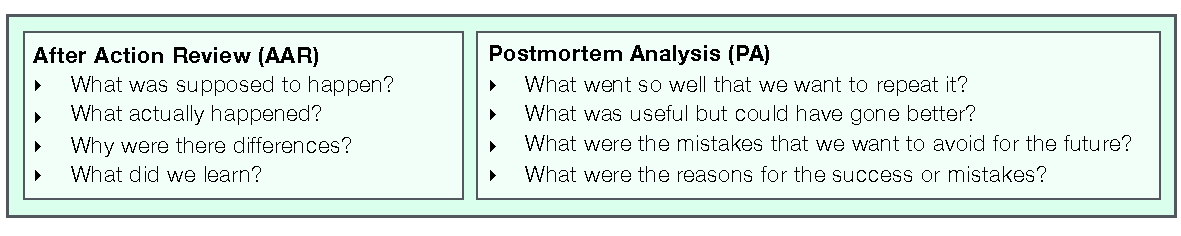
\includegraphics[width=12.5cm]{figures/aar_pma.pdf}
	\caption{\todo{text, sources}}
	\label{fig:aar_pma}
\end{figure}


\newpage
\section{Briefing Form}
TODO
	%\begin{itemize}
	\item in this paper we propose a one page briefing of research study
	\item supports EBSE and searchability of study
	\item similar to SEED but more detailed structure to support searchability even more.
	\item supports researcher in understanding the field of research
	\item supports researcher in understanding the study itself
	\item guides researcher through study design and result documentation process
	\item contains of: research question, hypothesis, experiment/context or deduction, conclusion
	\item experiment contains: independent and dependent variables (control variables), method, results  
\end{itemize}


\fbox{\begin{minipage}{\linewidth}
		{\large\textbf{Question}}\\
		Contains \textbf{\textit{technology}} in a \textbf{\textit{context}} showing an \textbf{\textit{effect}}. TODO Kitchenham Quote (practitioners)?\\
		\exampleQuote{Does pair programming in professional software development teams increases code quality?}
		\\
		\\
		\\
		{\large\textbf{Hypothesis}}\\
		Needs to contain a \textbf{\textit{prediction}} and needs to be \textbf{\textit{testable}}.\\
		\exampleQuote{If you do x, then y will happen}
		\\
		\\
		\\
		{\large\textbf{Experiment}}\\
		\textbf{Context}\\
		\\
		\textbf{Dependent Variables}\\
		Variables that are  \textbf{\textit{measured}} during the study.\\
		\\
		\textbf{Independent Variables}\\
		Variables that are  \textbf{\textit{changed}} during the study.\\
		\\
		\textbf{Method}\\
		Lab-/Field study, number of participants, metrics, ...\\
		\\
		\textbf{Results}\\
		Experiment's outcome\\
		\textbf{No} interpretation or conclusion!\\
		\\
		\\
		\\
		{\large\textbf{Conclusion}}\\
		Interpretation of experiment's results.\\
		Verifying or Falsifying Hypothesis.\\
		Scope of generalization.
\end{minipage}}
	\subsection{Research Question and Hypothesis}
\label{subsec:research question and hypothesis}

We decided to include both research question and hypothesis in the briefing form. Despite them being rather redundant in many cases. The research question is included due to the method researchers use to search for existing evidence, by entering their question into search engines. On the other side the hypothesis has its right to exist in the briefing form to support evaluation of validity and relevance of found evidence. \\
Therefore the fields in the form should be filled in with the research question and hypothesis constructed earlier (see section \ref{subsec:formulating research question and hypothesis}). The research question in a asking form which contains technology, context and effect. Or it is constructed according to the PICOT criteria. And the hypothesis in form of a testable prediction (e.g., \q{If [I do X], then [Y] will happen.} \cite{Buddies2010}).
	\subsection{Experiment}

TODO
		\subsubsection{Variables}

Variables are operationalizations of concepts, and there are usually three kinds of variables: Dependent, independent and controlled variables \cite{BuddiesVariables,Seltman2015}. A good variable must be measurable by any means \cite{BuddiesVariables}. Seltman additionally defines several qualities that make a good variable: \obsrvQuote{high reliability, absence of bias, low cost, practicability, objectivity, high acceptance, and high concept validity}\cite[p. 10]{Seltman2015}. \\

\todo{include classification of statistical type. has influence on choise of statistical method in experiment.}

We decided to include the different variables in the briefing form to make the decomposition of hypotheses easier while searching for related work. In order to make the search more fertile. Additionally the variables make it easier to evaluate the validity of the evidence.



\todo{maybe put this whole description part of experiment already in workflow and just state here that it is vital for the briefing.}

			\subsubsection{Independent Variables}
TODO
			\subsubsection{DependentVariables}
TODO

			% !TEX root = ../../seminar.tex

\paragraph{Controlled Variables}

The third variable category are controlled variables. They have or may have an effect on the dependent variables, but are not focus of the study. Therefore they are controlled by the researcher and kept constant throughout the experiment \cite{BuddiesVariables}. Examples for controlled variables in software engineering research are: the test environment of a software, the gender of participants, or the number of trials per group.
		\subsubsection{Research Techniques}

\begin{itemize}
	\item different techniques used in this experiment
	\item give examples
	\item why is this important in the brief?
\end{itemize}
		\subsubsection{Statistical Results}
\label{statisticalresults}

The outcome of an experiment is important for researchers who search for related work. Additionally the results help validating the solidity of evidence found. The statistic result of an experiment should never contain any interpretation. Interpretations should be given in a conclusion or discussion section separately from the data. //
This field should at least contain the used statistic measurement, method, or model and their resulting parameters (e.g. Analysis of Variance: F(2.57)=211.496, p<.001). It is advisable to use established methods to ensure comparability and reproducibility. More on statistical analysis can be found in books like \cite{Wohlin2012}, or \cite{Albert2008} as already mentioned in Section \ref{subsec:designing conducting and interpreting experiment}.

	% !TEX root = ../../seminar.tex

\subsection{Conclusion}
\label{subsec:conclusion}

This is the interesting part for searching researchers: What was found during the study? When searching for evidence researchers often like to see what question the study is about and what it finds. The conclusion indicates whether the question is answered or if more research has to be done on this issue. This includes an interpretation of the experiment results, and the verification or rejection of $H_0$ (and acceptance of $H_1$). Also a short statement on the scope of generalization should be given. Finally it must be clear if the given research question is answered and in which direction.

\newpage
% !TEX root = ../../seminar.tex

\section{Discussion}
\label{sec:discussion}

To support students in scientific working, this paper introduced a process along with guiding documents.
The process is mainly based on EBSE.\\
The workflow and documents were not evaluated in this work. Therefore, they need to be tested in future work. This should be done with students in real world scenarios such as bachelor and master theses. Comparing multiple theses is a difficult task. There are many influencing factors and already a certain variance in the quality of theses requiring a lot of subjects. Also finding a suiting metric to classify and compare two theses that might not be particularly similar is not trivial. Whereas asking students in a qualitative study can provide useful insight whether the documents were actually helpful or not.\\
When formatively evaluated, a digitalized version of \briefingform{} should be implemented to allow state of the art data collection and searching. This is a step towards an infrastructure which supports the use of EBSE on a larger scale. That kind of infrastructure might also be of interest for software practitioners and scientists.

%\bibliographystyle{splncs03}%
\bibliographystyle{alpha}%
\bibliography{seminar}%

\todo{append \briefingform and \checklist}
\end{document}
